\documentclass[10pt]{extarticle}
\usepackage[margin=0.68in]{geometry}
\usepackage{amsmath,amssymb,booktabs,array,tikz,xcolor,graphicx,pdflscape,hyperref}
\hypersetup{colorlinks=true,linkcolor=blue,urlcolor=blue}
\title{ISO-1 weak isogeny classes: trace census and a proved 2-adic obstruction}
\author{Research evidence report}
\date{8 October 2026}
\begin{document}
\special{pdf:minorversion 7}
\maketitle

\noindent\textbf{Requested scope.} Base primes $p=37$ through about $200$,
$q=p^2$, and curves over $\mathbb F_{q^3}=\mathbb F_{p^6}$: label every
full-2-torsion isogeny class and find a criterion for weak-class reach.
This round completed every-trace censuses at $p=37,41,43,47$ and diagnostic
censuses at $p=11,13,17$. It proves a necessary class obstruction for
every odd base prime. The other requested primes and an exact sufficient
criterion remain open.

\medskip
\noindent\textbf{Method.} A weak representative has
$y^2=x(x-\alpha)(x-\sigma\alpha)$, with $\sigma$ the $p^2$-Frobenius.
After translation and $\mathbb F_{p^2}$ square scaling there are
$2q^2+2q$ normalized representatives. The $p=37$ run evaluated one
representative per quadratic-twist pair and derived the opposite trace.
Trace assignment uses a randomized two-point baby-step/giant-step
counter. Its labels are computational evidence, not independent
certificates of every cardinality. Full and twist-derived CSVs agreed
exactly at $p=13$; two false individual assignments at $p=7$ were found
by exact square-table counting.
Independent PARI/GP \texttt{ellcard} checks placed 100, 3,952, 4,043,
and 4,200 distinct norm-one Legendre traces at $p=37,41,43,47$ in the
respective positive sets (5,000 samples each at $p=41,43,47$).

\begin{center}
\begin{tabular}{@{}r r r r r r r@{}}
\toprule
$p$ & $q$ & weak reps & ordinary $t$ & weak $t$ & depth-1 weak & depth-$\geq2$ zero \\
\midrule
11 & 121 & 29,524 & 1,210 & 542 & 0/606 & 62/604 \\
13 & 169 & 57,460 & 2,028 & 928 & 0/1,014 & 86/1,014 \\
17 & 289 & 167,620 & 4,624 & 2,198 & 0/2,312 & 114/2,312 \\
\textbf{37} & \textbf{1,369} & \textbf{3,751,060} & \textbf{49,284} & \textbf{24,352} & \textbf{0/24,642} & \textbf{290/24,642} \\
\textbf{41} & \textbf{1,681} & \textbf{5,654,884} & \textbf{67,240} & \textbf{33,224} & \textbf{0/33,620} & \textbf{396/33,620} \\
\textbf{43} & \textbf{1,849} & \textbf{6,841,300} & \textbf{77,658} & \textbf{38,452} & \textbf{0/38,830} & \textbf{376/38,828} \\
\textbf{47} & \textbf{2,209} & \textbf{9,763,780} & \textbf{101,614} & \textbf{50,382} & \textbf{0/50,808} & \textbf{424/50,806} \\
\bottomrule
\end{tabular}
\end{center}

\noindent At $p=37$ the run took 1,106.807 seconds with four Rayon
threads and counted 563,856,133,786 $\mathbb F_p$ multiplications.
The 50,654 CSV rows cover every candidate $t\equiv2\pmod4$ in the
Hasse interval; 49,284 are ordinary. Of 4,000 sampled random
full-2-torsion curves, 2,433 were in an observed weak class:
$0.6083$, Wilson 95\% interval $[0.5930,0.6233]$.
The zero-label share at $p=37$ is 50.59\% of ordinary trace rows but
39.18\% of sampled curves; these use different denominators. The
$p=41,43,47$ sampled reach fractions are $0.6253$, $0.6195$, and
$0.6320$ (4,000 curves each; Wilson 95\% intervals
$[0.6101,0.6401]$, $[0.6043,0.6344]$, and $[0.6169,0.6468]$).
At $p=47$ the special size-two orbit yields the two nonordinary
Hasse-boundary traces $t=\pm2\cdot47^3$ (two representatives each),
independently confirmed with PARI/GP.

\begin{center}
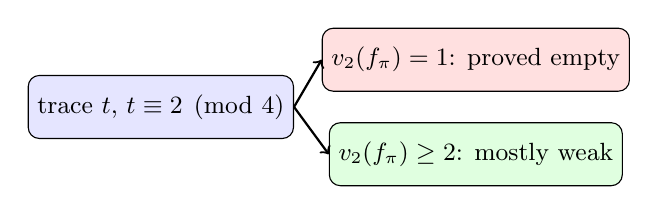
\begin{tikzpicture}[x=1cm,y=1cm, every node/.style={font=\small}]
\node[draw,rounded corners,fill=blue!10,minimum width=3.3cm,minimum height=0.8cm] (trace) at (0,0) {trace $t$, $t\equiv2\pmod4$};
\node[draw,rounded corners,fill=red!12,minimum width=3.2cm,minimum height=0.8cm] (low) at (4.0,0.6) {$v_2(f_\pi)=1$: proved empty};
\node[draw,rounded corners,fill=green!12,minimum width=3.2cm,minimum height=0.8cm] (high) at (4.0,-0.6) {$v_2(f_\pi)\geq2$: mostly weak};
\draw[->,thick] (trace.east) -- (low.west);
\draw[->,thick] (trace.east) -- (high.west);
\end{tikzpicture}
\end{center}

\clearpage
\noindent\textbf{Proof of the necessary obstruction.} Put
$K=\mathbb F_{p^6}$, $Q=p^6$, and
$\lambda=\alpha^{p^2}/\alpha$ on a weak model
$y^2=x(x-\alpha)(x-\alpha^{p^2})$.
Then $N_{K/\mathbb F_{p^2}}(\lambda)=1$, so $\lambda$ has odd order
dividing $p^4+p^2+1$. Since $p^2\equiv1\pmod4$, an explicit fourth root is
$\mu=\lambda^{(p^4+p^2+2)/4}$, with $\mu^4=\lambda$.
The weak curve is a quadratic twist of
$L_\lambda:y^2=x(x-1)(x-\lambda)$. The rational $2$-isogeny
at $(0,0)$ has target
\[
L'_\lambda:y^2=x\bigl[x^2+2(1+\lambda)x+(1-\lambda)^2\bigr],
\]
For $x\ne0$, the map is
\[
 (x,y)\longmapsto \left(x+a+\frac b x,\ y\left(1-\frac b{x^2}\right)\right),
 \qquad a=-(1+\lambda),\quad b=\lambda.
\]
The identity and $(0,0)$ map to the identity. With $U=x^2+ax+b$,
clearing the curve equations gives
$U^2-2axU+(a^2-4b)x^2=(x^2-b)^2$.
The target roots are $0,-(1+\mu^2)^2,-(1-\mu^2)^2$. All their differences
are squares: the final difference is $\pm4\mu^2$ and $-1$ is a
square in $K$. The roots are distinct since $\lambda\ne0,1$.
By \href{https://arxiv.org/pdf/math/0106273}{Auer--Top, Lemma 2.1},
each rational $2$-torsion point has a rational half, and the halves
of two independent points generate $L'_\lambda[4]$. Therefore
$16\mid\#L_\lambda(K)$, and the weak trace obeys
$t\equiv\pm(Q+1)\pmod{16}$.

\noindent Let
$t^2-4p^6=f_\pi^2D_K$, where $D_K$ is the fundamental CM
discriminant. The measured $v_2(f_\pi)$ is a class-wide bound, not
a certified endomorphism-ring volcano level. For ordinary
$t\equiv2\pmod4$, the arithmetic tests
\[
 v_2(f_\pi)\geq2\quad\Longleftrightarrow\quad
 (t/2)^2\equiv p^6\pmod{16}\quad\Longleftrightarrow\quad
 t/2\equiv\pm p^3\pmod8
\]
are equivalent to the proved trace restriction. Indeed,
$d=(t/2)^2-p^6$ has $v_2(d)\geq3$. If $v_2(d)=3$, then
$v_2(D_K)=3$ and $v_2(f_\pi)=1$; if $v_2(d)\geq4$, then
$v_2(t^2-4p^6)\geq6$ and $v_2(D_K)\in\{0,2,3\}$ forces
$v_2(f_\pi)\geq2$. Sufficiency fails on the recorded computational labels.
There is a curve-level consequence: on the 2-isogenous neighbor with
rational full $4$-torsion, $\pi-1$ factors through the separable map $[4]$.
Thus $\eta=(\pi-1)/4$ is an endomorphism, and
$\operatorname{disc}\mathbb Z[\eta]=(t_L^2-4p^6)/16$, where $t_L$ is
the untwisted Legendre trace. Its generated order has conductor $f_\pi/4$,
so the neighbor's endomorphism conductor has $2$-valuation at most $v_2(f_\pi)-2$.
Twisting preserves that order, and a degree-$2$ isogeny changes its
$2$-valuation by at most one (via the dual-isogeny inclusions of twice
each endomorphism ring). Thus an ordinary weak curve satisfies
$v_2(f_{\mathrm{End}(E)})\leq v_2(f_\pi)-1$: it is never at the deepest
possible $2$-volcano level. Individual levels remain unmeasured.
This bound also follows directly from full rational $2$-torsion:
$(\pi-1)/2$ is an endomorphism and its generated order has conductor
$f_\pi/2$. It applies to every full-$2$-torsion curve in the population,
so it does not further distinguish weak representatives. The extra class
restriction comes from full $4$-torsion on the neighbor.
The accompanying identity records replay the target factorization and
cleared isogeny equation at 32 recorded plus 64 additional points.
Independent exact PARI/GP expansion checks both identities over the integers;
the records cover those polynomial steps, while the theorem follows from
the deduction above.
The record IDs are \texttt{IDC1h8ae7209125dfe0a2} and
\texttt{IDC1he02ab9a5cf019a56}.
\newpage
\noindent\textbf{Held-out classifier.} On $p=37$ rows the necessary rule
has 24,352 true positives, 290 false positives, no false negatives,
and 24,642 true negatives (99.41\% correct); $p=41,43,47$ add 396,
376, and 424 false positives, respectively. At $p=47$, the necessary
rule has 99.58\% ordinary-row accuracy and no observed false negative.

\noindent\textbf{Counterexample to the proposed small invariants.}
At $p=37$, $t=-92{,}218$ has zero observed weak representatives and
$t=38{,}854$ has 24. Both have Frobenius conductor depth 3,
ramified 2, even maximal-order class number, and the same trace
modulo $2^{17}$. Their PARI/GP class numbers are 912 and 3,168.
Thus 2-splitting, conductor depth, small 2-power trace residues,
and class-number parity do not classify all rows together.
At $p=41$, traces $136542$ (zero) and $5470$ (132 weak representatives)
share depth 2, ramified 2, exact maximal-order class number $h_K=192$,
and the same trace modulo $2^{17}$. A near-edge pair, $133826$ (zero)
and $134082$ (12), shares depth 3, split 2, $h_K=1680$, and trace
modulo 256. Class-number magnitude is associated with residual zeros,
but does not yield an exact classifier even with these 2-adic features.
At held-out $p=47$, $t=204238$ (zero) and $t=73166$ (96) likewise share
depth 3, split 2, exact $h_K=336$, and trace modulo $2^{17}$.

\noindent\textbf{Exact orbit reduction and audit.} Projective $\alpha$
modulo $\mathbb F_q^*$ maps bijectively to the norm-one parameters
$\lambda\ne1$. Their $q$-Frobenius conjugates and inverses have the same
trace up to the quadratic twist already paired in the census. All such
orbits have size six except the nontrivial cube roots of unity, which
form one orbit of size two. Thus one point count per orbit suffices,
reducing the present algorithm's point-count calls by nearly sixfold.
At $p=13,37$ the orbit CSVs match the prior direct CSVs byte for byte;
$p=37$ needed 312,589 rather than 1,875,530 point counts. The corrected
$p=37,41,43,47$ counts obey the modulo-six constraint; at $p=47$ its
special pair is nonordinary. This structural
check is not an independent proof of every zero label.

\noindent\textbf{Where the residual zeros occur.} At $p=37$,
234 of 290 high-depth zero rows lie in the outer fifth of
$|t|/(2p^3)$ (234/4,930 rows there, versus 6/4,926 in the inner
fifth); $p=47$ has 392 of 424 residual zero rows in the outer fifth.
This is an association, not a causal proof or an exact rule.

\medskip
\noindent\textbf{Residual zeros and class-number magnitude.}
The population is ordinary positive traces with $v_2(f_\pi)\geq2$;
negative traces are their quadratic-twist mirrors. Native PARI/GP
\texttt{qfbclassno} gives $h_K$. Entries are zero labels / all traces in
each bin; the bins use $q=p^2$.
\begin{center}
\begingroup
\setlength{\tabcolsep}{8pt}
\begin{tabular}{@{}l r r r r r@{}}
\toprule
$h_K/q$ & $p=37$ & $p=41$ & $p=43$ & $p=47$ & combined \\
\midrule
$<1$ & 101/4,192 & 117/5,260 & 136/5,856 & 143/7,208 & 497/22,516 \\
$[1,2)$ & 30/2,518 & 52/3,347 & 30/3,817 & 41/4,776 & 153/14,458 \\
$[2,4)$ & 11/3,124 & 24/4,072 & 22/4,582 & 25/5,829 & 82/17,607 \\
$[4,8)$ & 3/2,365 & 5/3,790 & 0/4,654 & 3/6,511 & 11/17,320 \\
$\geq8$ & 0/122 & 0/341 & 0/505 & 0/1,079 & 0/2,047 \\
\bottomrule
\end{tabular}
\endgroup
\end{center}
\noindent These are complete observed strata, not sampled rates.
The matched pairs above rule out using the listed features as an exact
classifier of the recorded labels. Independent certification of every
zero label remains open.

\medskip
\noindent\textbf{Correction to prior evidence.} The earlier census
used an $\mathbb F_p$ nonsquare for the second
$\mathbb F_{p^2}$ square class. Every nonzero element of $\mathbb F_p$
is a square in $\mathbb F_{p^2}$, so it duplicated one branch and
omitted the other. The corrected code selects a genuine
$\mathbb F_{p^2}$ nonsquare. Old $p\leq31$ values remain historical;
$p=23,31$ await corrected reruns.

\noindent\textbf{Limit.} At $p=199$, twist symmetry needs 1,568,278,802
point counts; the exact orbit quotient reduces this to 261,379,801.
Scaling the measured $p=37$ direct run by work count and the approximate
$p^{3/2}$ cost per point count gives roughly 130 days for the older
method on comparable resources. This is a crude extrapolation, not a
run, and excludes growing trace-factorization work.
The requested $p=53$--200 census and a sufficient replacement formula
have not been established. The theorem certifies absence in about half
of the candidate classes and can safely prefilter them.

\medskip
\noindent\textbf{Evidence.} The accompanying Markdown report links
the code, complete CSVs, fit output, samples, and SVG. The $p=37$ command used
\texttt{RAYON\_NUM\_THREADS=4} and \texttt{--derive-twists}.
The weak-model and reach assumptions are in
\href{https://eprint.iacr.org/2011/020.pdf}{Joux--Vitse, \S4.1};
\href{https://arxiv.org/abs/math/0106273}{Auer--Top} proves a
broader Legendre-family statement.
The accompanying \href{REPORT.md}{Markdown report} links every CSV,
the identity records, and the new validation receipt.

\clearpage
\begin{landscape}
\begin{center}
\textbf{Complete observed trace strata and invariant flow}\\[1ex]
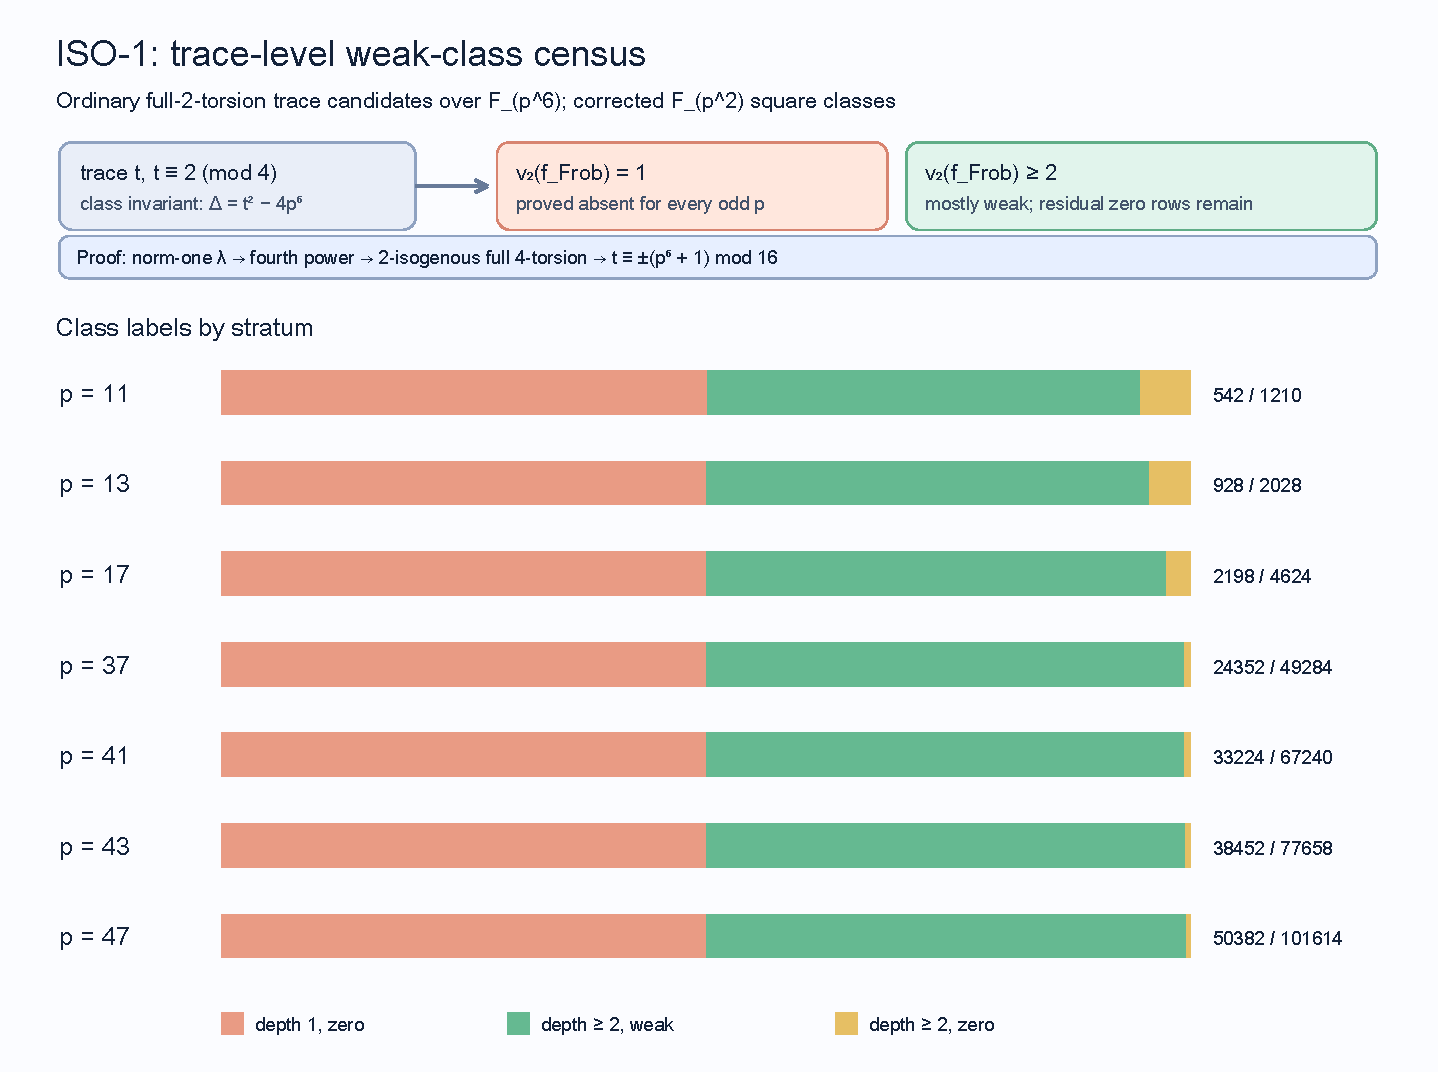
\includegraphics[width=\linewidth,height=0.85\textheight,keepaspectratio]{class_strata.pdf}
\end{center}
\noindent Source: the seven census CSVs linked in the Markdown report,
rendered by \texttt{iso1\_class\_census visual}. The bars count ordinary
trace rows; their widths are fractions of each prime's row population.
The right-hand labels give weak rows / ordinary rows. Sampling intervals
apply to the separate 4,000-curve reach samples, not these census bars.
The proof excludes every depth-1 class; the yellow segments retain the
observed high-depth zero rows and their point-count uncertainty.
\end{landscape}
\end{document}
